\documentclass[twocolumn,superscriptaddress]{revtex4-1}
\usepackage{graphicx}
\usepackage{amsmath}
% \usepackage{hyperref}
\usepackage{booktabs}
\usepackage{color}
\usepackage{multirow}
\setlength{\tabcolsep}{10pt}

\usepackage{pgfplots}
\usepgfplotslibrary{external}
\usepgfplotslibrary{groupplots}
\usepackage{pgfplotstable}
\usetikzlibrary{positioning}
\usetikzlibrary{plotmarks}
\usetikzlibrary{patterns}
\usetikzlibrary{matrix}
\tikzexternalize
\tikzsetexternalprefix{fig_}
\tikzset{external/force remake=false}
\tikzset{every mark/.append style={scale=0.8}}
\pgfplotsset{every axis/.append style={small}}

\pgfplotscreateplotcyclelist{grade5}{%
blue, every mark/.append style={fill=blue},mark=*\\%
blue!30!gray,every mark/.append style={fill=blue!30!gray},mark=square*\\%
gray!50!black,mark=star\\%
red!30!gray, every mark/.append style={fill=red!30!gray}, mark=triangle*\\%
red, every mark/.append style={fill=red},mark=diamond*\\%
}

\begin{document}

\tikzset{external/force remake=false}
\tikzsetnextfilename{distrib}
\begin{figure}
	\centering
	\begin{tikzpicture}
	\begin{groupplot}[%
		group style={
			group size=2 by 3,
			horizontal sep=0.01\textwidth,
			y descriptions at=edge left,
			},%
		width=0.325\columnwidth,%
		height=0.325\columnwidth,%
		axis y line=left,
		axis x line*=bottom,
		xlabel near ticks,
		xlabel shift=-0.5em,
		ylabel near ticks,
		scale only axis,
		axis on top,
		ymode=log,%
		no markers,%
		every axis plot post/.append style={red, dashed},
		]
		\nextgroupplot[xlabel=$s_2$, xmin=-70,xmax=0]
		\fill[gray!20] (axis cs:-70,1e-7) rectangle (axis cs:-29.34,1);
		\addplot file{s2_distrib_mobility};
		
		\nextgroupplot[xlabel=$f_2$, xmin=0,xmax=25]
		\fill[gray!20] (axis cs:11.98,1e-7) rectangle (axis cs:25,1);
		\addplot file{f2_distrib_mobility};
		
		\nextgroupplot[xlabel=$q_6$, xmin=0,xmax=0.8, ylabel={Probability}]
		\fill[gray!20] (axis cs:0.495,1e-7) rectangle (axis cs:0.8,1);
		\addplot file{q6_distrib_mobility};
		
		\nextgroupplot[xlabel=$100w_6$, xmin=-5.2,xmax=1]
		\fill[gray!20] (axis cs:-5.2,1e-7) rectangle (axis cs:-1.44,1);
		\addplot table[x expr=\thisrowno{0}*100]{w6_distrib_mobility};
		
		\nextgroupplot[xlabel=$Q_6$, xmin=0,xmax=0.6]
		\fill[gray!20] (axis cs:0.234,1e-7) rectangle (axis cs:0.6,1);
		\addplot file{Q6_distrib_mobility};
		
		\nextgroupplot[xlabel=$C$, xmin=-6,xmax=12]
		\fill[gray!20] (axis cs:5.11,1e-7) rectangle (axis cs:12,1);
		\addplot file{C_distrib_mobility};
	\end{groupplot}
	\begin{groupplot}[%
		group style={
			group size=2 by 3,
			horizontal sep=0.01\textwidth,
			y descriptions at=edge right,
			},%
		width=0.325\columnwidth,%
		height=0.325\columnwidth,%
		ymin=0,ymax=2,%
		no markers,
		axis y line=right,
		axis x line=none,
		ylabel near ticks,
		scale only axis,
		extra y ticks={1}, extra y tick labels={}, extra tick style={grid=major},%
		]
		\nextgroupplot[xlabel=$s_2$, xmin=-70,xmax=0]
		\addplot table[x index=0, y index=2]{s2_distrib_mobility};
		
		\nextgroupplot[xlabel=$f_2$, xmin=0,xmax=25]
		\addplot table[x index=0, y index=2]{f2_distrib_mobility};
		
		\nextgroupplot[xlabel=$q_6$, xmin=0,xmax=0.8]
		\addplot table[x index=0, y index=2]{q6_distrib_mobility};
		
		\nextgroupplot[xlabel=$w_6$, xmin=-5.2,xmax=1, ylabel={Mobility}]
		\addplot table[x expr=\thisrowno{0}*100, y index=2]{w6_distrib_mobility};
		
		\nextgroupplot[xlabel=$Q_6$, xmin=0,xmax=0.6]
		\addplot table[x index=0, y index=2]{Q6_distrib_mobility};
		
		\nextgroupplot[xlabel=$C$, xmin=-6,xmax=12]
		\addplot table[x index=0, y index=2]{C_distrib_mobility};
	\end{groupplot}
	\end{tikzpicture}
	\caption{\textbf{Probability distribution} (red dash) \textbf{and mobility} (blue continuous) function of various order parameter at $\beta p\sigma^3=25$ and for a time difference corresponding to the $\alpha$-relaxation. Mobility is in unit of mean-square displacement. The limit of the shaded area is at one standard deviation from the mean value of the order parameter in the direction of ordering.}
	\label{fig:distrib}
\end{figure}

\tikzset{external/force remake=false}
\tikzsetnextfilename{structurefactor}
\begin{figure}
	\centering
	\begin{tikzpicture}
	\pgfplotsset{fitc/.style={solid, no markers, forget plot, domain=0.05:5}}
	\begin{groupplot}[%
		group style={
			group size=1 by 2,
			horizontal sep=0.1\textwidth,
			},%
		width=0.9\columnwidth,
		height=0.4\columnwidth,%
		xlabel near ticks,
		xlabel shift=-0.5em,
		ylabel near ticks,
		xmode=log,
		ymode=log,%
		ytickten={-1,0,1}, yticklabels={0.1,~~1,10},
		cycle list name=grade5,%
		legend style={at={(0.5,1.03)}, anchor=south},
		legend columns=10,
		]
		\nextgroupplot[%
			xlabel={$q\xi_{f_2}$}, ylabel={$S_{f_2}(q)/\chi_{f_2}$},
			xmin=0.05,xmax=2,%
			ymin=0.5, ymax=1.5, 
			]
			\addlegendimage{empty legend}
			%\addlegendimage{legend image code/.code={\node[right] {$P=$};}};
			%\addlegendentry{};
			\addplot+[only marks] table[x expr={0.076*\coordindex}, y expr={\thisrowno{0}/0.186}] {Sf2-std_P17};
			\addplot+[only marks] table[x expr={0.0764*\coordindex}, y expr={\thisrowno{0}/0.176}] {Sf2-std_P19};
			\addplot+[only marks] table[x expr={0.0742*\coordindex}, y expr={\thisrowno{0}/0.178}] {Sf2-std_P21};
			\addplot+[only marks] table[x expr={0.0751*\coordindex}, y expr={\thisrowno{0}/0.178}] {Sf2-std_P23};
			\addplot+[only marks] table[x expr={0.0731*\coordindex}, y expr={\thisrowno{0}/0.173}] {Sf2-std_P25};
			\addplot+[black, fitc] {1/(1+x^2)};
			\legend{Pressures, $17$, $19$, $21$, $23$, $25$};
		
		\nextgroupplot[
			xlabel={$q\xi_{Q_6}$}, ylabel={$S_{Q_6}(q)/\chi_{Q_6}$},%
			xmin=0.1,xmax=10,%
			ymin=0.02, ymax=2,%
			]
			\addplot+[only marks] table[x expr={0.338*\coordindex}, y expr={\thisrowno{0}/0.937}] {SC-std_P17};
			\addplot+[only marks] table[x expr={0.373*\coordindex}, y expr={\thisrowno{0}/1.22}] {SC-std_P19};
			\addplot+[only marks] table[x expr={0.412*\coordindex}, y expr={\thisrowno{0}/1.32}] {SC-std_P21};
			\addplot+[only marks] table[x expr={0.471*\coordindex}, y expr={\thisrowno{0}/1.61}] {SC-std_P23};
			\addplot+[only marks] table[x expr={0.533*\coordindex}, y expr={\thisrowno{0}/2.23}] {SC-std_P25};
			\addplot+[black, fitc] {1/(1+x^2)};
			
	\end{groupplot}
	\end{tikzpicture}
	\caption{\textbf{Structure factors} collapse on the Ornstein-Zernike form for (top) $f_2$ and (bottom) $C$. Note how the former are almost similar across pressures.}
	\label{fig:structurefactor}
\end{figure}

\tikzset{external/force remake=false}
\tikzsetnextfilename{lengths}
\begin{figure}
	\centering
	\begin{tikzpicture}
	\pgfplotsset{every axis/.append style={
		height=0.6\columnwidth,%
		width=0.95\columnwidth,
		cycle list name=exotic,
		xlabel={$\beta p\sigma^3$},
		ymin=0,
		xmin=8,
		xtick={9,13,...,25},
	}}
	\begin{axis}[%
		name=len,
		ylabel={$\xi_x$},
		ymax=1.6,
		legend style={at={(1,1.03)}, anchor=south east},
		legend columns=10,
		]
	\pgfplotstableread{lengths}\lengths
	 \foreach \y in {1, 2, ..., 6} {
          \addplot table[x index=0, y index=\y]{\lengths};
          \pgfplotstablegetcolumnnamebyindex{\y}\of{\lengths}\to{\colname}
          \addlegendentryexpanded{$\colname$}
          }
	\end{axis}
	\begin{axis}[%
		at={(len.below south west)},
		anchor=above north west,
		ylabel={$\chi_x$},
		ymax=2,
		]
	\pgfplotstableread{susceptibilities}\sus
	 \foreach \y in {1, 2, ..., 6} {
          \addplot table[x index=0, y index=\y]{\sus};
          \pgfplotstablegetcolumnnamebyindex{\y}\of{\sus}\to{\colname}
          }
	\end{axis}
	\end{tikzpicture}
	\caption{\textbf{Correlation length} extracted for two-body and multi-body scalar order parameters, function of the pressure.}
	\label{fig:lengths}
\end{figure}

\tikzset{external/force remake=false}
\tikzsetnextfilename{polydistrib}
\begin{figure}
	\centering
	\begin{tikzpicture}
	\pgfplotstableread{w6_poly.hist}\wtable
	\pgfplotstableread{Q6_poly.hist}\Qtable
	\begin{groupplot}[%
		group style={
			group name=di,
			group size=1 by 2,
			horizontal sep=0.1\textwidth,
			},%
		width=0.95\columnwidth,
		height=0.6\columnwidth,%
		xlabel near ticks,
		xlabel shift=-0.5em,
		ylabel near ticks,
		ymode=log,%
		cycle list name=grade5,%
		no marks,
		legend style={at={(0.5,1.05)}, anchor=south},
		legend columns=10,
		]
		\nextgroupplot[xlabel=$100w_6$, xlabel=$100w_6$, xmin=-5.2,xmax=-2,		ymin= 1e-6,ymax=1e-2, ylabel=$P(w_6)$]
		\addlegendimage{empty legend}
		\foreach \y in {1, 2, ..., 5} {
          \addplot table[x expr=\thisrowno{0}*100, y index=\y]{\wtable};
          }
        \node at (axis cs:-2.25,8e-6) (a) {};
        \legend{$\Delta$, $0.07$, $0.09$, $0.11$, $0.13$, $0.15$};
        \draw (axis cs:-4.4,7e-5) node[right] {$\Delta$} [->]  -- (axis cs:-4.75,2e-4);
        
		\nextgroupplot[xlabel=$Q_6$, xmin=0,xmax=0.5, xtick={0,0.1,...,0.5}, ylabel=$P(Q_6)$]
		\addlegendimage{empty legend}
		\foreach \y in {1, 2, ..., 5} {
          \addplot table[y index=\y]{\Qtable};
          }
        \draw (axis cs:0.4,1e-4) node[right] {$\Delta$} [->]  -- (axis cs:0.3,1e-5);
	\end{groupplot}
	\begin{axis}[%
		at={(a)},
		anchor=south east,
		width=0.425\columnwidth,
		xlabel=$100w_6$, xmin=-5.2,xmax=1,
		xlabel near ticks,
		xlabel shift=-0.5em,
		ylabel=$P(w_6)$,
		ylabel near ticks,
		ymode=log,%
		cycle list name=grade5,%
		no marks,
		]
		\foreach \y in {1, 2, ..., 5} {
          \addplot table[x expr=\thisrowno{0}*100, y index=\y]{\wtable};
          }
	\end{axis}
	\end{tikzpicture}
	\caption{\textbf{Effect of polydispersity} on local structures at constant pressure ($\beta p\sigma^3=23$). \textbf{top} detail of the distribution of $w_6$ (full distribution in inset) showing a small increase in the icosahedra population saturating around $10\%$. \textbf{bottom} distribution of $Q_6$ showing a marked decrease in the crystallinity.}
	\label{fig:polydistrib}
\end{figure}

\tikzset{external/force remake=false}
\tikzsetnextfilename{f2decoupling}
\begin{figure}
	\begin{tikzpicture}[
		lab/.append style={below right}%,
		]%
		\pgfplotsset{
			extra tick style={grid=major, major grid style={
				copy shadow={very thick, shadow xshift=0, shadow yshift=0, white, semitransparent}, 
				black}},%
		}
		\begin{groupplot}[
			group style={
				group name=X,
				group size=2 by 1,%
				horizontal sep=0.075\textwidth,
				},%
			width=0.525\columnwidth,%
			height=0.525\columnwidth,
			ylabel={$f_2$},%
			ymin=0,ymax=25,%
			enlargelimits=false,axis on top,
			xlabel near ticks,
			ylabel near ticks,
			]
		\nextgroupplot[%
			xlabel=$Q_6$,%
			xmin=0,xmax=0.6,%
			]
			\addplot graphics
				[xmin=0,xmax=0.6,ymin=0,ymax=25]
				{f2_Q6_hist.png};
		
		\nextgroupplot[%
			xlabel=$100w_6$,%
			xmin=-5.2,xmax=1,%
			]
			\addplot graphics
				[xmin=-5.2,xmax=5.2,ymin=0,ymax=25]
				{f2_w6_hist.png};		
		\end{groupplot}
		\path (X c1r1.north east) -- (X c2r1.north west) node[midway] (T) {};
		
%		%%color scales by hand
		\matrix (l1) [above=0.5em of T, matrix anchor=south, matrix of nodes, minimum width=2em, minimum height=1em, inner sep=0, draw=black]
		{
			|[fill=white]| & 
			|[fill=black!20!white]| &
			|[fill=black!40!white]| &
			|[fill=black!60!white]| &
			|[fill=black!80!white]| &
			|[fill=black]| \\
		};
		\node[above, at=(l1-1-1.north east)] {$10^1$};
		\node[above, at=(l1-1-2.north east)] {$10^2$};
		\node[above, at=(l1-1-3.north east)] {$10^3$};
		\node[above, at=(l1-1-4.north east)] {$10^4$};
		\node[above, at=(l1-1-5.north east)] {$10^5$};
		%\node[below, at=(l1-1-3.south east)] {$Probability$};
	\end{tikzpicture}
	\caption{\textbf{Correlation between two-body and multi-body parameters.} Probability distribution functions in the $f_2$,$Q_6$-map (top) and in the $f_2$,$w_6$-map (bottom) for a metastable fluid with polydispersity $\Delta=7\%$ and pressure $\beta p\sigma^3=23$. The parameters are not correlated, even in extreme values.}
	\label{fig:f2decoupling}
\end{figure}

\tikzset{external/force remake=false}
\tikzsetnextfilename{Cmaps}
\begin{figure}
	\begin{tikzpicture}
	\begin{groupplot}[
			group style={
				group name=X,
				group size=2 by 1,%
				horizontal sep=0.075\textwidth,
				},%
			width=0.525\columnwidth,%
			height=0.525\columnwidth,
			xlabel=$q_4$,%
			xmin=0,xmax=0.3,%
			ylabel={$q_6$},%
			ymin=0,ymax=0.7,%
			enlargelimits=false,axis on top,
			xlabel near ticks,
			ylabel near ticks,
			]
		\nextgroupplot
			\addplot graphics
				[xmin=0,xmax=0.3,ymin=0,ymax=0.7]
				{q4_q6_C_s07.png};
		\nextgroupplot
			\addplot graphics
				[xmin=0,xmax=0.3,ymin=0,ymax=0.7]
				{q4_q6_C_s15.png};
	\end{groupplot}
	\path (X c1r1.north east) -- (X c2r1.north west) node[midway] (T) {};
	\begin{axis}[%
		name=B,
		anchor=below south, at=(T.north),
		width = 0.6\columnwidth,
		height= 1em,
		xmin=-4, xmax=12, ymin=0, ymax=1,
		xtick={-4,-2,...,12},
		axis y line=none,
		axis x line*=none,
		scale only axis,
		axis on top,
		]
		\addplot graphics
			[xmin=-4,xmax=12, ymin=0, ymax=1]{colorscale.png};
	\end{axis}
	\node[left=0.5em of B] {$C(q_4,q_6)$};
	%\node[above=0.5em of T] {
\includegraphics{colorscale.png}};
	\end{tikzpicture}
	\caption{Average crystallinity order parameter projected in the $q_4$,$q_6$ space for the metastable fluid at $\beta p\sigma^3=23$ at $\Delta=7\%$ (top) and $\Delta=15\%$. Icosahedra appear in the top-left corner of each plot and perfect \textsc{fcc} crystals would be in the top-right corner.}
	\label{fig:Cmaps}
\end{figure}

\tikzset{external/force remake=false}
\tikzsetnextfilename{3D}
\begin{figure}
	\begin{tikzpicture}
	\matrix[matrix of nodes]{
		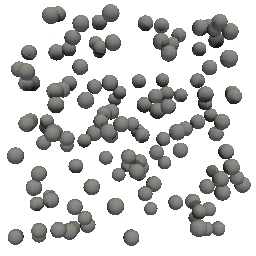
\includegraphics[width=0.45\columnwidth]{s2_slice_3D} & 
		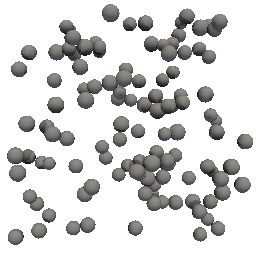
\includegraphics[width=0.45\columnwidth]{f2_slice_3D} \\
		$s_2$ & $f_2$ \\
		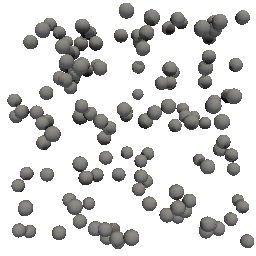
\includegraphics[width=0.45\columnwidth]{q6_slice_3D} & 
		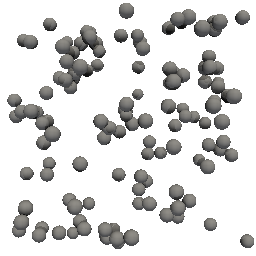
\includegraphics[width=0.45\columnwidth]{w6_slice_3D} \\
		$q_6$ & $w_6$ \\
		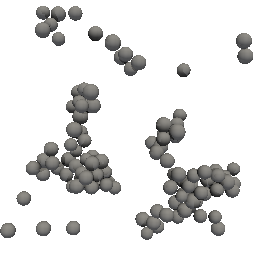
\includegraphics[width=0.45\columnwidth]{Q6_slice_3D} & 
		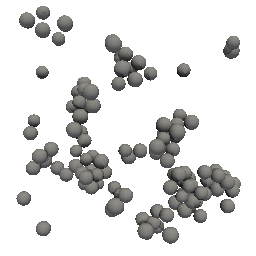
\includegraphics[width=0.45\columnwidth]{C_slice_3D} \\
		$Q_6$ & $C$ \\
	};
	\end{tikzpicture}
	\caption{\textbf{Visualisation of the ordered regions} defined by the various order parameters. All pictures correspond to a thin slice ($5\sigma$) of the same configuration at $\beta p\sigma^3=23$ and $\Delta=7\%$. Only $Q_6$ and $C$ show meaningful fluctuations.}
	\label{fig:3D}
\end{figure}

\tikzset{external/force remake=false}
\tikzsetnextfilename{lengthpoly}
\begin{figure}
	\begin{tikzpicture}
	\begin{axis}[%
		height=0.5\columnwidth,
		xlabel={$\Delta$ (\%)},
		ylabel={$\xi_x$},
		xmin=6,ymin=0,
		xtick={7,9,...,15},
		reverse legend=true,
		legend style={
			legend pos=outer north east,
			}
		]
		\addplot+[black, mark=diamond] table[y index=2]{f2-std_P23.chixi};
		\addplot+[blue, mark options={fill=blue}] table[y index=2]{w6-std_P23.chixi};
		\addplot+[red] table[y index=2]{Q6-std_P23.chixi};
		\legend{$f_2$,$w_6$,$Q_6$};
	\end{axis}
	\end{tikzpicture}
	\caption{\textbf{Polydispersity dependence of the correlation lengths} at $\beta p\sigma^3=23$. The dominant crystalline length decreases, the icosahedral length increases, however they plateau well before crossing. The two-body length shows no indication of becoming dominant with increasing $\Delta$, even decreasing slightly.}
	\label{fig:lengthpoly}
\end{figure}

\tikzset{external/force remake}
\tikzsetnextfilename{eos}
\begin{figure}
	\begin{tikzpicture}
	\begin{axis}[%
		width=0.95\columnwidth,
		height=0.5\columnwidth,
		xlabel={$\phi$},
		ylabel={$\beta p\sigma^3$},
		xmin=0.45, xmax=0.59,
		ytick={9,11,...,27},
		]
		\addplot file{figures/fig1/circles.dat};
		\addplot+[every mark/.append style={scale=0.8}, mark=square
] file{figures/fig1/squares.dat};
		\addplot[mark=diamond] coordinates {(0.5347,17) (0.5358, 17) (0.537528, 17)};
		%\addplot[domain=0.45:0.59, dashed] {(1+x+x^2-x^3)/(1-x)^3};
	\end{axis}
	\end{tikzpicture}
	\caption{Simulated state points. The circles (blue curve) represent the equation of state for polydispersity $\Delta=7\%$. The squares (red curve) instead are simulation points at the same pressure ($\beta p\sigma^3=23$) but at different polydispersities $\Delta$: from low to high volume fraction they correspond to $\Delta=7\%,9\%,11\%,13\%,15\%$ respectively. Similarly the diamonds (black curve) are at $\beta p\sigma^3=17$ and $\Delta=0\%,4\%,7\%$.}
	\label{fig:eos}
\end{figure}

\tikzset{external/force remake=false}
\tikzsetnextfilename{stability_map}
\begin{figure}
	\begin{tikzpicture}
	\begin{axis}[%
		width=0.95\columnwidth,
		height=0.5\columnwidth,
		xlabel={$q_6$},
		ylabel={$\phi$},
		%ymax=0.62,
		xmin=0.45, xmax=0.58,
		no marks,
		axis on top,
		legend style={
			legend pos=north west,
		}
		]
		\addplot+[black, very thick] file{figures/fig7/crystalline.dat};
		\addplot file{figures/fig7/d0.dat};
		\addplot+[dashed, blue] file{figures/fig7/d4.dat};
		\legend{crystalline,$\Delta=0\%$,$\Delta=4\%$};
	\end{axis}
	\end{tikzpicture}
	 \caption{Average $\phi$ as a function of $q_6$ for particles identified as fluid and crystalline. The continuous red curve represents fluid particles in a system at $\beta p\sigma^3=17$ and $\Delta=0\%$, while dashed blue curve represents fluid particles at the same pressure but at $\Delta=4\%$. The thick black curve represents instead solid particles (this curve is less sensitive to polydispersity and it is reported once).}
 \label{fig:stability_map}
\end{figure}
\end{document}